%%%%%%%%%%%%%%%%%%%%%%%%%%%%%%%%%%%%%%%%%%%%%%%%%%%%%%%%%%%%%%%%%%%
%                                                                 %
%   ZEBRA User Guide -- LaTeX Source                              %
%                                                                 %
%   Chapter Introduction                                          %
%                                                                 %
%   The following external EPS files are referenced:              %
%   linstru , genstru , zeblink , bnkform , relocat               %
%                                                                 %
%   Editor: Michel Goossens / CN-AS                               %
%   Last Mod.:  7 Jun. 1993 07:30  mg                             %
%                                                                 %
%%%%%%%%%%%%%%%%%%%%%%%%%%%%%%%%%%%%%%%%%%%%%%%%%%%%%%%%%%%%%%%%%%%

\Filename{H1ZEBRA-An-overview}

\chapter{ZEBRA - An overview}

\Filename{H2Intro-Why-ZEBRA}
\section{Why ZEBRA?}

All off-line programming in high-energy physics is carried out, for
various reasons, in the Fortran~77 programming language. While this
language offers certain advantages over its competitors, it does suffer
from one serious defect, namely its lack of dynamic data structuring
facilities. The only data structures it contains at all are the array of
homogeneous elements and the common block for shared data. Neither of
these structures can be manipulated as an entity, and neither of them
can be defined dynamically at execution-time. No pointers are available
to link these structures together at a higher level.
If we were to attempt to
define structures using standard Fortran they would thus, at best, be in
the following style:

\begin{XMPt}{Example of defining data structure with Fortran}
      PARAMETER (NTRACKS = 100 , NPTS = 20)
      COMMON/POINTS/PTRACK(3,NTRACK),XYZ(NPTS,NTRACK),...
\end{XMPt}

and almost the whole program would have to be regenerated and recompiled
every time one of the symbolic constants is altered.
Relationships between data items would have to be programmed explicitly
using integer arrays of indices.
 
It is to overcome these limitations that the ZEBRA system has been
designed and written. It allows not only a truely dynamic
creation of data structures at execution-time, but also the added
advantage of being able to
{\bf manipulate} those structures, and even to write them to an external
storage medium and to recover them intact on some other computer.
In order to achieve this, the
user has to communicate with the ZEBRA system by (mostly) simple calls
to ZEBRA routines, and by following a number of rules and conventions.
Once a program has been written in this fashion, it becomes easy
for anyone knowing rather few of the details to use and to modify the
program, without having to worry about the side-effects of any changes
he or she makes, and without having to recompile large sections of the
code solely in order to obtain a few extra storage locations.
 
ZEBRA provides a significant extension to the power of Fortran, in
general at an insignificant cost in terms of execution-time overheads.
However, even that small cost is tiny compared with the extra time which
would otherwise be wasted in developing large programs using only the
conventional facilities.
 
The purpose of this chapter is to introduce the novice user to the basic
terms and concepts of ZEBRA. The actual use of the system
is described in later
chapters, where all the relevant information on calling sequences and so
forth is set out.

\Filename{H2Intro-Logical-Data-Structures}
\section{Logical Data Structures}
\subsection{The bank}

Imagine that we wish to store all the information about, say, a track in
a single unit, containing perhaps details of its momentum, direction,
coordinates etc. Using a call to the ZEBRA routine \Rind{MZBOOK}, we can ask
for an area of contiguous storage of a given length to be provided. The
actual location of this area is returned by \Rind{MZBOOK} as a
{\bf base address} which has to be used in all references to that area.
\index{bank}
This unit of storage is called a
{\bf bank}, and in Fortran code will be referenced as in:
\begin{XMPt}{Addressing data words in a ZEBRA bank}
      Q(LTK+1) = PX
      Q(LTK+2) = PY
      etc.
\end{XMPt}
\Lit{Q}, by convention, is the name of the Fortran array underlying the
data structure, and \Lit{LTK} is the base address,
provided by \Rind{MZBOOK}, being the location of the word
preceding the first data word in the bank.
 
An advantage of ZEBRA is that it allows banks to contain data of
differing types. This is explained in detail later, but a simple
application would allow us to address another data word in the bank just
referenced as an integer, e.g.
\begin{XMPt}{Addressing integer data in a ZEBRA bank}
      IQ(LTK+19) = NPOINTS
\end{XMPt}
It is important to understand that for data structuring purposes
ZEBRA requires no knowledge of or control
over the actual contents of a bank. 
Whether it contains track data or a
list of family birthdays is not ZEBRA's concern. 
The internal details of
the data in a bank are solely the responsibility of the user(s), and it is
vital to maintain an adequate documentation of bank contents.
However, for input/output across computers and for printing
purposes, ZEBRA has to know the type of the bank contents, i.e. whether
the numbers are floating point, integer, Hollerith, etc.
This can be declared by a call to \Rind{MZFORM}.

\subsection{The linear structure}

In our example of a track bank, it is clear that in a given application
there may be a large and variable number of tracks to deal with.
To permit the realization of sets of objects of the same kind, ZEBRA
provides the construct of the {\bf linear structure} (figure \ref{LINSTRU}).
A linear structure consists of a series of linked banks, with each bank
holding in a reserved system word, called the {\bf next link},
the base address of the next member of the set. The next link of the
last bank of a linear structure has the value zero, indicating that
there is no next bank.
\index{link!next}
\index{data structure!linear}

\begin{minipage}{\textwidth}

\begin{Fighere}
\begin{center}
\mbox{\epsfig{file=linstru.eps,width=.9\textwidth}}
\end{center}
\caption{A simple linear structure}
\label{LINSTRU}
\end{Fighere}

\vspace*{-2mm}

\begin{XMPt}{Example of loop over linear chain}
      LTK = LFIRST                      ! Address of the first bank
   10 IF (LTK.EQ.0) GO TO finished      ! No next bank left ?
            .....                       ! Process data for the bank at LTK
          LTK = LQ(LTK)                 ! Get the address of the next bank
      GO TO 10                          ! Loop
\end{XMPt}
\end{minipage}

\newpage

The next link is stored in the word \Lit{LQ(LTK)} of the bank,
with the vector \Lit{LQ}
in offset EQUIVALENCE to the vector \Lit{Q} and \Lit{IQ}, as explained later.
The example above shows the ZEBRA equivalent of a Fortran DO-loop to process
all the banks of a linear structure.

Banks are created dynamically at execution time, and because each
bank has one word to connect the rest of the structure of which it is a
member, the linear structure permits the creation at
execution time of sets of an arbitrary number of objects,
independent of any declaration of maximum dimension, either at
execution time or at compile time, as would be the case with Fortran
arrays.

The order of the banks in a linear structure, although defined, is not
normally significant. It depends on the details of the creation process,
as will be seen later. The user may, however, associate significance to
the defined order, and ZEBRA utilities are provided to re-order the
banks in a linear structure by re-arranging the next links (\Rind{ZSORT}).

It will be necessary to refer to the
``address of a linear structure''.
This is simply the base address of its first bank. If this address is
available, all the banks of the linear structure can be reached.
\subsection{The general data structure}
\index{data structure!general}
\index{link!down}

In the general case, more complex structures are needed than the linear
one just described. 

\begin{Fighere}
\begin{center}
\mbox{\epsfig{file=genstru.eps,width=\textwidth}}
\end{center}
\caption{An example of a general structure}
\label{GENSTRC}
\end{Fighere}

For instance, in the context of a high-energy
physics program a number of track banks may depend on a bank at a
logically higher level which
describes a track vertex. 
This vertex bank will
contain a link to the first of the track banks. 
Such a link is called a {\bf down} link.
It is possible for a given bank to have a large number of
down links, and for it to depend similarly on a logically yet higher bank
through a down link in that bank.
We thus see that the down links allow the construction of
a tree structure, and that at each node there may be either a
single bank or a linear structure. This may be pictured as in
Figure~\ref{GENSTRC}.

All the links so far described are stored by ZEBRA as part of the bank
concerned. We note that the down and next links are referred to collectively
as {\bf structural} links, as they represent the basic connections
of a data structure.

\subsection{Reverse links}

Each ZEBRA bank contains a link pointing to the bank on which the
whole linear structure of which it is a member depends. 
This is called the {\bf up link}. 
The value of this link is zero if the bank concerned is 
itself at the top of the tree structure.
Finally, each bank has also an {\bf origin} link, which points
to the structural link supporting the bank.
The up link and the origin link are known as {\bf reverse} links.
A summary of the four types of links known to ZEBRA is given in
Figure \ref{ZEBLINK}\index{link!reverse}
\index{link!origin}
\index{link!up}

\subsection{Reference links}

The links so far described are an integral part of the data structure
which they represent. It often happens that a user wishes to establish
links between various banks which are not part of the structure itself,
but merely references that the user wishes to record.
These are then known as
{\bf reference links}. A bank can contain a large number of such links,
and their use is at the discretion of the user, and entirely his
responsiblity. For the reference links the task of
the ZEBRA system is limited to changing their
values in the event that, for reasons to be explained
below, banks have to be moved, or relocated, in memory. Reference links
provide a high level of generality in the design of complete data
structures, and are another of those features which so greatly
enhances the power of Fortran.

\begin{Fighere}
\begin{center}
\mbox{\epsfig{file=zeblink.eps,width=\textwidth}}
\end{center}
\caption{A schematic overview of the links known to ZEBRA}
\label{ZEBLINK}
\end{Fighere}

\Filename{H2Intro-Physical-Storage}
\section{Physical Storage}

It is clear that somehow the banks just described have to be mapped on
to physical computer storage, or memory.
This is achieved in ZEBRA by declaring to the system one or more common
blocks which are to provide the actual storage for the data structures.
It is often sufficient for off-line programs to declare a single large
common block; it is for on-line applications, or for certain large
off-line applications that the possibility to define several distinct
blocks is foreseen. A typical declaration has the following form:
\begin{XMPt}{Declaration of the ZEBRA storage}
      COMMON /MYSTOR/ IFENCE(10),LINKS(10),LINKR(20),ISTORE(10000)
      DIMENSION     LQ(999),IQ(999),Q(999)
      EQUIVALENCE  (LINKS(9),LQ(9),IQ(1),Q(1))
\end{XMPt}
An actual common block is declared to ZEBRA by a call to \Rind{MZSTOR},
and in ZEBRA is termed a {\bf dynamic store}.
The actual layout of memory in a store declared by the example above is shown
in figure \ref{FMZSTOR}.

\begin{Fighere}
\begin{center}
\mbox{\epsfig{file=mzstor.eps,width=\textwidth}}
\end{center}
\caption{The layout of the ZEBRA default store}
\label{FMZSTOR}
\end{Fighere}

Within the common block just described, we notice that the effect of th
\Lit{EQUIVALENCE} statement is to offset the arrays \Lit{Q} and 
\Lit{LQ} by eight locations. 
This permits in the references to the data words and to the
links a simple form of subscript, namely that each data word is
addressed as \Lit{Q(L+n)}, 
as already seen, and that each link is referenced as \Lit{LQ(L-m)}. 
This may be better appreciated by studying the layout of an
actual bank, whose layout is detailed in Figure~\ref{BNKFORM},
where the various sections of the bank may be seen, in particular the
data and the links.

\begin{figure}[p]
\begin{center}
\mbox{\epsfig{file=bnkform.eps,width=\textwidth}}
\end{center}
\caption{The format of a ZEBRA bank}
\label{BNKFORM}
\end{figure}

The total number of links \Lit{NL} plus a constant plus the number of the
optional, so-called extra I/O words, stored
in the lower part of the first word of the bank (see below),
is required to step over the link
region to reach the central area during a sequential scan
through the store.
The upper part of the first word contains the I/O control-byte.
Together with the extra I/O words, if any, it constitutes the
``I/O characteristic'', describing the nature of the bank contents,
as needed for conversion if the bank is written to a file for reading
on some other computer, and also for interpretative dumps
(see the description of routine \Rind{MZFORM}).
\index{bank!I/O characteristic}
\index{link!next}
\index{link!up}
\index{link!origin}

The central part of the bank starts with the next link,
accessed as \Lit{LQ(L)}.
The up link at \Lit{LQ(L+1)} points to the header bank supporting
the linear structure of which the bank is a member;
it is zero if the bank is a primary header bank.
The origin link at \Lit{LQ(L+2)} points to the link
through which the bank is reached.
The origin link is not usually of interest to the user,
its sole purpose is to free the user from having to remember the
supporting link. These three links, next, up and origin are present
in every bank and are not counted in \Lit{NL} and \Lit{NS}.
\index{bank!identifier!numeric}
\index{bank!identifier!Hollerith}

The two words \Lit{IQ(L-5)} and \Lit{IQ(L-4)} contain the numeric and Hollerith bank
identifiers, \Lit{IDN} and \Lit{IDH}. 
Usually all the banks of a linear structure
have the same \Lit{IDH}, but different \Lit{IDN}'s to permit ready
identification of a particular bank in interactive work.
Words \Lit{IQ(L-3)} and \Lit{IQ(L-2)}
hold the total number of links (\Lit{NL}) and the number of structural
links (\Lit{NS}), respectively,
and word \Lit{IQ(L-1)} holds the number of data words (\Lit{ND}).

The status word at \Lit{IQ(L)} provides in positions
1 to 18 for user status bits,
while positions 19 to 32 are reserved for system use. In particular
bits 19 to 22 contain the number of extra I/O descriptor words \Lit{NIO},
needed to go backwards from the centre to the start of a bank.

With this format the smallest possible, but useless, ZEBRA
bank (\Lit{NL=NS=ND=0}) occupies 10 words.

\subsection{Divisions}
\index{division}

So far we have seen how banks are stored in a dynamic
store. In fact, a dynamic store may physically be subdivided into
{\bf divisions}. The purpose of the division is to enable ZEBRA to
manipulate groups of logically associated banks efficiently, for instance
for input-output or for dropping banks, and also to allow it to handle links
more efficiently when it knows that they are restricted to a single
division.

When a store is initialized by \Rind{MZSTOR}, it automatically creates three
divisions, one for itself and two for the user. Further divisions may be
created explicitly by a call to \Rind{MZDIV}.

It should be noted that stores and divisions are identified by
means of a store/division index whose value never changes. These indices
should be maintained in, for instance, the common block to which they
refer, for reasons of
data integrity.

\subsection{Link areas}
\index{link!area}

It is possible for a user to store bank addresses or links, for ease
of manipulation, in a user-defined area, or {\bf link area}.
These should be kept in a common block, and a call to
\Rind{MZLINK} or \Rind{MZLINT} is necessary to declare these areas to ZEBRA, which
will then maintain them in the event of a bank relocation. For this
reason, the link areas associated with different stores have to be kept
separately.

\subsection{Working space}
\index{working space}

It happens frequently in a program that some temporary working space is
required, perhaps for use within one or two routines. 
ZEBRA permits a user to ask for such working space by a call to \Rind{MZWORK}. 
The necessary
storage is made physically available at the beginning of the relevant
store, and may contain reference links and data. It should be noted that
the first division in the store is logically part of the working space,
and its existing contents are destroyed by a call to \Rind{MZWORK}. 
Normally, therefore, the first division should itself be used only for 
banks which are very short term.

\newpage
\Filename{H2Intro-Dropping-banks-and-garbage-collection}
\section{Dropping banks and garbage collection}

Initially a dynamic store is empty, except for a few system banks in the
system division. As banks are created the occupied space increases and
the free space decreases. 
By calling \Rind{MZDROP} the user may {\bf drop}
banks, which are not needed any longer. 
\Rind{MZDROP} logically removes banks,
or whole sub-structures, from the surrounding data structure and marks
the banks as dropped. These dropped banks stay intact in memory and in
particular, reference links pointing to dropped banks continue to point
to valid information.
\index{garbage collection}

Possibly, but not normally, the situation can arise, that the free space
is not sufficient to satisfy a request for creating a bank, in which case
ZEBRA will recuperate the space occupied by the dropped banks. 
This operation, called {\bf garbage collection}, moves the active
banks of
a division to form one contiguous area, squeezing out the dropped banks
and thereby increasing again the free space, updating all links for the
new positions of the banks in memory, including a reset to zero of
reference links which used to point to the dropped banks which have now
disappeared. The process of changing the links for the new position in
memory is called {\bf relocation}.
\index{relocation}

ZEBRA triggers a garbage collection automatically whenever a request
for memory cannot be satisfied. If even after garbage collection there
is not enough space, \Rind{MZBOOK} etc. will take an error exit and thus the
user does not have to test, after each call to \Rind{MZBOOK} etc., for the
successful completion of the request.

For garbage collection the ZEBRA system has to know the whereabouts of
{\bf all} the links in the program. 
For this reason it
is essential that the user keeps all bank addresses in locations known
to ZEBRA, either in the link part of banks, or in the link part of the
working space or in link areas. 
Any link kept elsewhere will be invalid after a garbage collection.
 
The memory move involved in a garbage collection is represented in
Figure~\ref{RELOCAT}.

\vspace*{-5mm}
\begin{Fighere}
\begin{center}
\mbox{\epsfig{file=relocat.eps,width=\textwidth}}
\end{center}
\caption[The layout of memory in a division before and after garbage
         collection.]%
        {The layout of memory in a division before and after garbage
collection.\\ The top part of the picture
shows a number of ``live'' banks numbered 1 to 7
and 5' to 1', which interspersed ``dead''
banks (i.e. banks whose information is no longer needed and whose space
can hence be recovered).
The bottom part of the picture shows the same ``live''
banks which have been left justified to increase the free space.}
\label{RELOCAT}
\end{Fighere}

\newpage
\Filename{H2Intro-Wiping-divisions}
\section{Wiping divisions}

In high energy physics repetitive ``event processing''
is a very common
situation: event-by-event the data are read, processed, output and
dropped. Each event is represented by one or several data structures,
which disappear completely before the next event is dealt with.
In this situation it would be inefficient to drop the event with \Rind{MZDROP}
and to rely on garbage collection to recover the space of the previous
event only later, maybe at the moment when the data volume of the new
event is already substantial and would have to be copied. It is much
more efficient to separate the short term data of the event from the
long term data (data held by the program over many events), by
directing them into separate divisions. The event can then be
abandoned with \Rind{MZWIPE} which resets one or several divisions to be empty,
thereby freeing the space for immediate re-use.

\Filename{H2Intro-Input-Output}
\section{Input/Output}

One of the important features of ZEBRA is its ability to handle the
transfer of data structures to and from an external medium. 
This is performed by calls to routines in the FZ part of the
\index{FZ!Sequential input/output}\index{input/output!FZ}%
system, and the user does not need to program any explicit Fortran input/output
statements. 
But the power of the system goes beyond that of a simple data transfer. 
It is able to maintain the integrity of a data structure
between an output operation and a subsequent input operation by
appropriate changes to the values of the links connecting the structure. 
In addition, ZEBRA permits input/output to either sequential or direct 
access files, depending on the nature
of the data and, very important, it also provides two modes of data
representation. 
\index{FZ!Sequential input/output!native mode}%
The first is called {\bf native} mode, and implies that the data 
undergo no conversion when
transfered between storage and the external medium. Such data may be read
only on a computer of a compatible architecture. 
The {\bf exchange} mode, on the other hand,
\index{FZ!Sequential input/output!exchange mode}%
allows transfer of data between a large variety of
computers by making appropriate conversions to and from an interchange
format.
                                          
On the other hand the ZEBRA RZ package permits the storage and retrieval of 
ZEBRA data structures or Fortran vectors in random access files. 
Files may reside on standard
direct access devices such as magnetic disk, or be
mapped to virtual memory. 
\RZfile s can be accessed by several users simultaneously,
even across networks.
Remote file access and transfer is provided for RZ files
using standard tools, such as NFS and ftp. In the heterogeneous
environment, the tools provided in the CSPACK~\cite{bib-CSPACK} 
package may be used.

The RZ package is not a relational database management system,
but organises data in a hierarchical manner which is suitable
for many applications in High Energy Physics, and probably outside.


\newpage
\Filename{H2Intro-Debugging-problems}
\section{Debugging problems}
\subsection{The debugging and documentation package}

It is inevitable that errors will sometimes be made in constructing and
manipulating the data structures supported by ZEBRA. 
In order to allow
a simple and convenient means of checking the integrity of the structures,
including the links and the data, the DZ package has been provided
(see chapter \ref{sec:dzdescription}.
It has various options to display and validate the whole or part of a dynamic
store.

The DZDOC package contains routines for generating and maintaining documentation
on ZEBRA data structures (see chapter~\ref{sec:dzdocdescription}).

\subsection{The user communication array {\tt IQUEST}}

Information about problems or important input/output running
parameters is available in the user communication array 
\IQUEST{} in common \Lit{/\QUEST/}. 
In order to have access to the information in this array
the user should include the following definition in his code:
\begin{XMPt}{Fortran definition of the user communication vector \Lit{IQUEST}}
      COMMON /QUEST/IQUEST(100)
\end{XMPt}
When a routine detects an error, it identifies itself and gives the
case number describing the problem. 
This number, together with the
detailed description of the contents of the \IQUEST{} elements, will allow
the user to trace the problem.

In the case of input/output routines (i.e. the FZ and RZ packages)
information about the last operation is available via \IQUEST{}
(see the description of each routine for the meaning of individual 
\IQUEST{} values).

\Filename{H2Intro-Some-conventions}
\section{Some conventions}

ZEBRA uses certain conventions,
for instance that the second letter of each routine or common block
name is a \Lit{Q} or \Lit{Z}. 
For this reason, users are urged not to
write common block or routine names which could be confused with ZEBRA
names, by avoiding these two letters in that position. 
Users are also
recommended to begin all link names with an \Lit{L}, in order that this become
a common convention, thereby improving the readability of programs.

\Filename{H2Intro-Summary}
\section{Summary}

This chapter has tried to set out the basic features of ZEBRA, together
with a justification for attempting to increase the power of the
programming facilities available to a programmer in this way. The nature
of the data structures has been described, together with the manner
in which they
can be manipulated, displayed, and written and read.

The ZEBRA system has been developed, in part, because of weaknesses in
Fortran 77. 
The new language standard Fortran~90 provides high level data structure
constructs, whose impact on high-energy physics programming are being
investigated.
Until then, high-energy physicists are able
to develop data structures, one of the most important parts of
programming, using ZEBRA.
